155. \begin{figure}[ht!]
\center{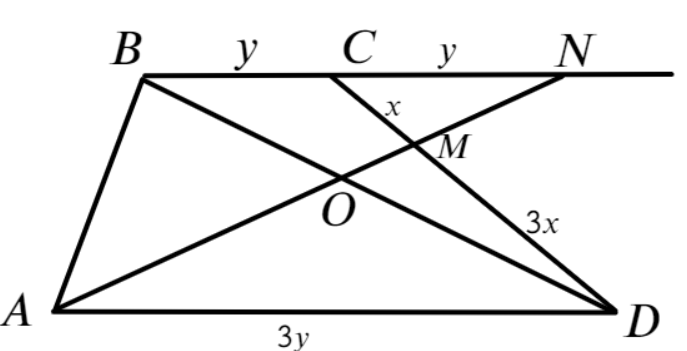
\includegraphics[scale=0.35]{g9-155.png}}
\end{figure}\\
Обозначим $CM=x,\ DM=3x,\ BC=y,\ AD=3y.$ Продлим $AM$ до пересечения с продолжением $BC$ в точке $N.$ Треугольники $CMN$ и $AMD$ подобны по двум углам (накрест лежащие  $MCN$ с $MDA$ и $MNC$ с $MAD$, значит $\cfrac{CN}{AD}=\cfrac{CM}{DM}=\cfrac{1}{3},\ CN=y.$ Тогда $BN=y+y=2y=\cfrac{2}{3}AD$ и треугольники $OBN$ и $ODA$ подобны двум углам (накрест лежащие $OBN$ с $ODA$ и $ONB$ с $OAD),$ поэтому $\cfrac{BO}{OD}=\cfrac{BN}{AD}=\cfrac{2}{3}$ и $BO:OD=2:3,$ а также $2AO=3ON.$ Из подобия треугольников $CMN$ и $AMD$ получаем $AM=3MN.$ Значит, $MN=\cfrac{1}{4}AN,$ а $AO=\cfrac{3}{5}AN,$ поэтому $OM=AN-AO-MN=\cfrac{3}{20}AN.$ Таким образом, $AO:OM=\cfrac{3}{5}AN:\cfrac{3}{20}AN=4:1.$\\
